\documentclass[twoside,11pt]{report}

% Any additional packages needed should be included after jmlr2e.
% Note that jmlr2e.sty includes epsfig, amssymb, natbib and graphicx,
% and defines many common macros, such as 'proof' and 'example'.
%
% It also sets the bibliographystyle to plainnat; for more information on
% natbib citation styles, see the natbib documentation, a copy of which
% is archived at http://www.jmlr.org/format/natbib.pdf

\usepackage{jmlr2e}
% \usepackage[utf8]{inputenc}%
% \usepackage{tikz}
% \usepackage{cfr-lm}%
\usepackage[T1]{fontenc}%
\usepackage{physics}
\usepackage{amsmath}
% \usepackage{amssymb}
% \usepackage{graphicx}
% \usepackage[margin=3cm]{geometry}
% \usepackage{changepage}
\usepackage{fontspec}
\usepackage{minted}
\usepackage{tcolorbox}
\usepackage{lmodern}
\usepackage{xcolor}
\usepackage{lettrine}
% \usepackage{fontawesome}
\usemintedstyle{perldoc}
\usepackage{hyperref}
\hypersetup{colorlinks=false, pdfborder={0 0 0},  }
\usepackage{fancyhdr}
\usepackage{wrapfig}
\usepackage{adjustbox}
\usepackage{tikz}
\usepackage{listofitems} % for \readlist to create arrays



\newtcbox{\codebox}[1][black]{on line, arc=2pt,colback=#1!10!white,colframe=white, before upper={\rule[-3pt]{0pt}{10pt}},boxrule=1pt, boxsep=0pt,left=2pt,right=2pt,top=1pt,bottom=.5pt}
\newtcbox{\deloppg}[1][black]{on line, arc=2pt,colback=#1!10!white,colframe=white, before upper={\rule[-2pt]{0pt}{0pt}},boxrule=0pt, boxsep=0pt,left=.49\linewidth,right=.49\linewidth,top=4pt,bottom=3pt}


\newcommand\blfootnote[1]{ \begingroup \renewcommand\thefootnote{}\footnote{#1} \addtocounter{footnote}{-1} \endgroup }
% \definecolor{antwhite}{HTML}{323333}
\newcommand{\code}[3][]{\codebox{\mintinline[#1]{#2}{#3}}}



% \setmainfont{FreeSans}
% \setmainfont{SF Pro Display}
% \setmainfont{IBM Plex Sans}
% \setmainfont{TeX Gyre Heros}
% \setmainfont{Inter}
% \setmainfont{Iosevka Quasi}
% \setmainfont{DM Sans}

% \setmonofont{Iosevka Custom Extended}
% \setmonofont{JetBrainsMono Nerd Font}
\setmonofont[Scale=MatchLowercase]{DM Mono}





% Definitions of handy macros can go here

\newcommand{\dataset}{{\cal D}}
\newcommand{\fracpartial}[2]{\frac{\partial #1}{\partial  #2}}

% Heading arguments are {volume}{year}{pages}{submitted}{published}{author-full-names}

% \jmlrheading{1}{2000}{1-48}{4/00}{10/00}{https://github.com/bragewiseth/MachineLearningProjects}

% Short headings should be running head and authors last names

\ShortHeadings{\url{https://github.com/bragewiseth/MachineLearningProjects}}{\url{https://github.com/bragewiseth/MachineLearningProjects}}
\firstpageno{1}



\title{{\huge Project 2}}
\author{\name Brage W. \email bragewi@ifi.uio.no\\
    \name Felix C. H.  \email felixch@ifi.uio.no \\
\name Eirik B. J. \email eiribja@ifi.uio.no}
\date{\today}											% Date
\makeatletter






% \date{\today}

\begin{document}

%%%%%%%%%%%%%%%%%%%%%%%%%%%%%%%%%%%%%%%%%%%%%%%%%%%%%%%%%%%%%%%%%%%%%%%%%%%%%%%%%%%%%%%%%

\begin{titlepage}
    \centering
    \vspace*{0.5 cm}
    
\includegraphics[scale = 0.75]{uio.jpg}\\[1.0 cm]	% University Logo
    \textsc{\LARGE University of Oslo}\\[2.0 cm]	    % University Name
    \textsc{\Large FYS-STK3155}\\[0.5 cm]				% Course Code
    \rule{\linewidth}{0.2 mm} \\[0.4 cm]
    { \huge \bfseries \@title}\\
    \rule{\linewidth}{0.2 mm} \\[1.5 cm]

    \begin{minipage}{0.4\textwidth}
        \begin{flushleft} \normalsize
            Brage Wiseth\\
            Felix Cameren Heyerdahl\\
            Eirik Bjørnson Jahr\\
        \end{flushleft}
    \end{minipage}~
    \begin{minipage}{0.4\textwidth}
        \begin{flushright} \normalsize
            \textsc{
                bragewi@ifi.uio.no\\
                felixch@ifi.uio.no\\
                eiribja@ifi.uio.no\\
            }
        \end{flushright}

    \end{minipage}\\[2 cm]
    \@date\\
    \vspace*{25mm}
    \urlstyle{rm}
    \textsc{\url{https://github.com/bragewiseth/MachineLearningProjects}}







\end{titlepage}
\nocite{*}
% \maketitle
\newpage
\tableofcontents
\newpage




\begin{abstract}%   <- trailing '%' for backward compatibility of .sty file
    \lettrine{I}{}n this paper, we delve into the realm of machine learning model optimization
    and evaluation. Our study encompasses various regression techniques, including 
    Ordinary Least Squares (OLS), Ridge, and Lasso regression, to analyze their effectiveness in handling
    simple and more complex datasets. Additionally, we employ bootstrap resampling and cross-validation
    methodologies to rigorously assess model performance and enhance generalization. A significant portion
    of our investigation is dedicated to understanding the delicate balance between bias and variance. 
    We explore how regularization methods like Ridge and Lasso impact bias-variance trade-offs, 
    offering insights into the stability and predictive power of these models. Furthermore, we provide
    empirical evidence of the benefits of cross-validation and bootstrap techniques in mitigating 
    overfitting and improving model robustness. We found that \{ ..results.. \}. Additionally we verify
    and compare our findings with well established theory and libraris such as SKLearn.
\end{abstract}
\begin{keywords}
    Linear Regression, Scaling, Bias \& Variance 
\end{keywords}









\section{Introduction}

An overview

\textbf{Gradient Decent}: 

\textbf{Data}: 

\textbf{Results}:

\textbf{Conclusion}:\\

In project 1\cite{MachineLearningProjects_2023}, we found that 
we can fit lines or even polynimals that approximate the distribution of our data by solving an nice analytical expression for the optimal parameters $\beta$. We can in principle approximate 
any function with a polynomial, if we give ourselves infinite degrees of freedom. This is great but there are several
limitations to this approach. First of all, we can not give ourselves infinite degrees of freedom, believe it or not.
Secondly, what if we don't want to find a polynimal but rather classify our data into some classes?\\

To tackle classification we can use \emph{logistic regression}, that is, first regression and then clamp the output to a binary value
(for the bianry case). We can do this with an activation function like the sigmoid function
\footnote{The sigmoid function does not output a binary value, but a value between 0 and 1. 
    We can then set a threshold, for example 0.5, and say that if the output is above the threshold, 
    we classify it as 1, and if it is below, we classify it as 0. We can interpret the output as the probability of the data point being 1.}
or the heaviside function. However the first problem
still remains, we want to approximate any function, but don't want to use an infinite taylor series. 
We need a different approach.
Instead of finding a single high degree polynimial, we can try to glue together a bunch of smaller line segments.
For this we can use a \emph{neural network}.
As it turns out, the framework for neural networks is very similar to the framework for logistic regression.
Neural networks can be interpeted as several logistic regression models glued together, which is exactly what we wanted!
Another huge benefit of this is that we can use the same code
For both logistic and linear regression as well as neural networks.

This sounds great, but by introducing activation functions we lose the nice analytical expression,
so we can't use the same matrix inversion approach as before.\\
So how do we learn?







\begin{center}
    \scriptsize code for generating all figures and data can be found at 
    \href{https://github.com/bragewiseth/MachineLearningProjects/tree/main/project1/src}{\tt \textsc{/MachineLearningProjects/project1/src} }
\end{center}




\section{ Gradient Descent }
\label{sec:GD}


\subsection{ Backpropagation and Chain Rule }
\label{sec:backpropagation}


\begin{figure}[!h]
    \begin{center}
        Forward\\
        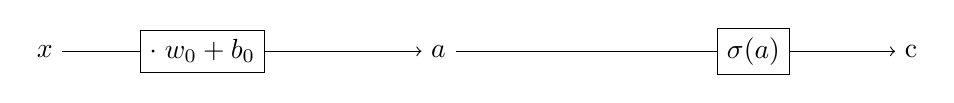
\begin{tikzpicture}
            \node (a) at (1,0) {$x$};
            \node (b) at (6,0) {$a$};
            \node (c) at (12,0) {c};
            \node[draw] (box1) at (3,0) {$\cdot\; w_0 + b_0$}; 
            \node[draw] (box2) at (10,0) {$\sigma(a)$};
            \draw[-] (a) -- (box1);
            \draw[->] (box1) -- (b); 
            \draw[-] (b) -- (box2);
            \draw[->] (box2) -- (c);
        \end{tikzpicture}\\
        Backwards\\
        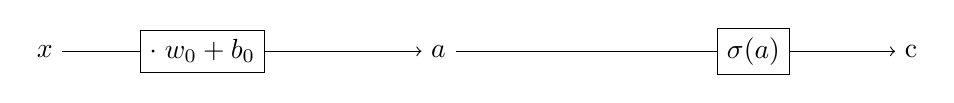
\begin{tikzpicture}
            \node (a) at (1,0) {$x$};
            \node (b) at (6,0) {$a$};
            \node (c) at (12,0) {c};
            \node[draw] (box1) at (3,0) {$\cdot\; w_0 + b_0$}; 
            \node[draw] (box2) at (10,0) {$\sigma(a)$};
            \draw[-] (a) -- (box1);
            \draw[->] (box1) -- (b); 
            \draw[-] (b) -- (box2);
            \draw[->] (box2) -- (c);
        \end{tikzpicture}
    \end{center}
    \caption{chain rule}\label{fig:chainrule}
\end{figure}






\section{ Neural Network }
\label{sec:NN}

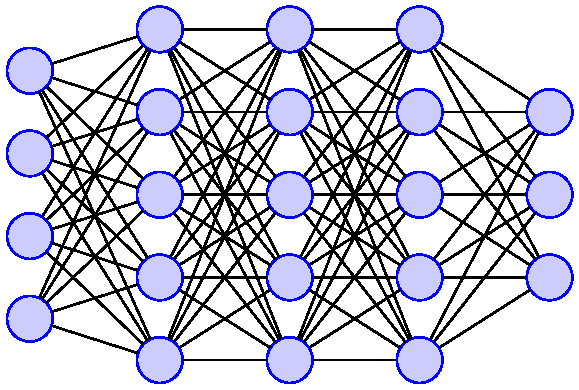
\includegraphics[width=\linewidth]{nn.pdf}

with one layer the network becomes a linear regression model. $y = x_0w_0 + x_1w_1 + x_2w_2 + ... + x_nw_n + b_0$ with a activation function at the end we can make it into a logistig regression model.
This makes it very convenient to use the same code for both linear and logistic regression as well as for 
larger neural networks with hidden layers, by simply swapping out the different parts.


\section{ Universal Approximation Theorem }
\label{sec:UAT}

There is a famous theorem called the universal approximation theorem, which states that a neural network with one hidden
layer can approximate any function. This is great, but it does not say anything about how many neurons we need in the
hidden layer. It turns out that we need an infinite number of neurons to approximate any function. This is not very
practical, so we need to find a way to approximate any function with a finite number of neurons.\\

Geofry Hinton showed that a simple perceptron is incapable of learning the XOR function. 
This is because the perceptron is a linear model, and the XOR function is not linearly separable. 
However, as we hinted at earlier, we can approximate any function with a polynomial or a neural network.


\section{Data}
\label{sec:data}






% The data we will be using consists of 100 points generated using the Franke function. The Franke function is a weighted sum of four exponentials given by
% \begin{align*}
%     f(x,y) &= \frac{3}{4}\exp\left(-\frac{(9x-2)^2}{4}-\frac{(9y-2)^2}{4}\right)\\
%     &+ \frac{3}{4}\exp\left(-\frac{(9x+1)^2}{49}-\frac{(9y+1)}{10}\right)\\
%     &+ \frac{1}{2}\exp\left(-\frac{(9x-7)^2}{4}-\frac{(9y-3)^2}{4}\right)\\
%     &- \frac{1}{5}\exp\left(-(9x-4)^2-(9y-7)^2\right)
% \end{align*}
% We will add some noise to the data to better simulate real world data. The data is generated by sampling $x$ and $y$ from a uniform distribution on the interval $[0,1]$. The noise is sampled from a normal distribution with mean 0 and standard deviation $\sigma = 0.1$.
% \begin{figure}[!h]
% \begin{minipage}[!t]{.48\linewidth}
%     \begin{center}
%         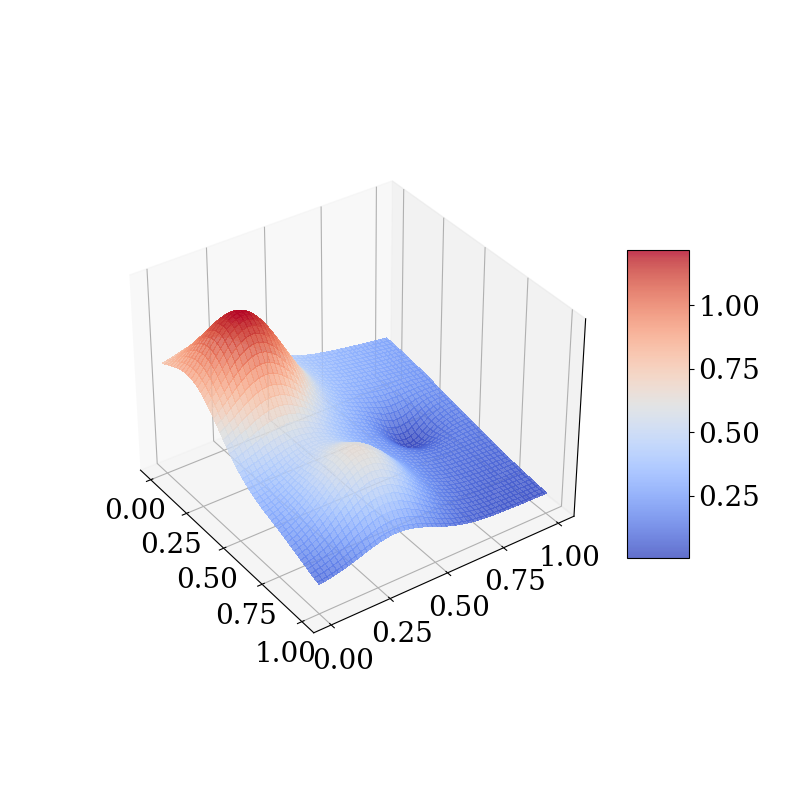
\includegraphics[width=1.1\textwidth]{../runsAndAdditions/trueFunction.png}
%         \caption{True Function}\label{fig:truefunction}
% \end{center}
% \end{minipage}
% \hspace{2mm}
% \begin{minipage}[!t]{.48\linewidth}
%     \begin{center}
%         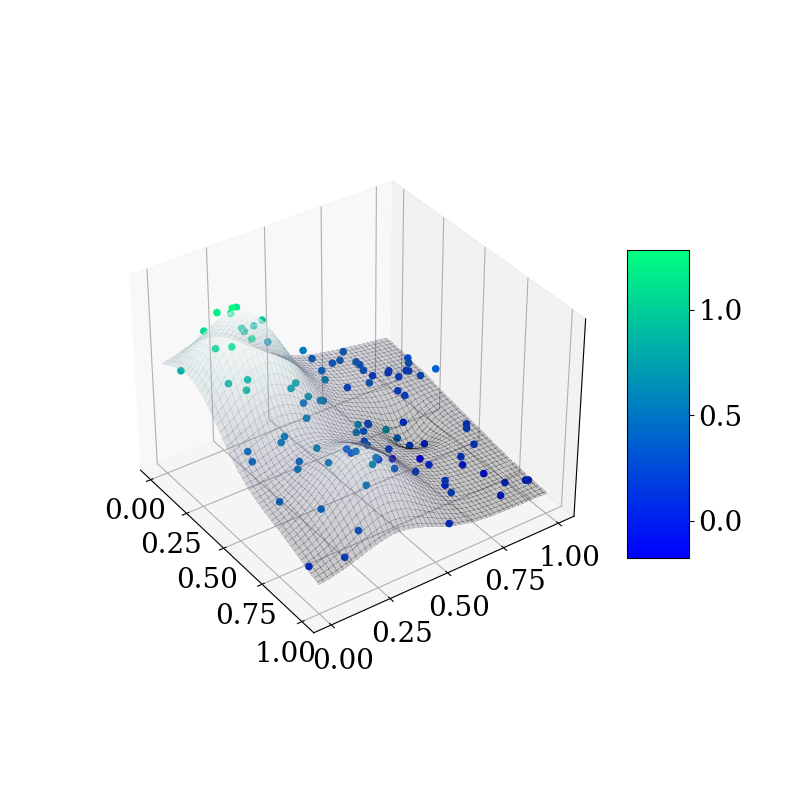
\includegraphics[width=1.1\textwidth]{../runsAndAdditions/synthDataSide.png}
%         \caption{Our Synthetic Data}\label{fig:synthdataside}
%     \end{center}
% \end{minipage}
% \end{figure}
% \begin{figure}[!h]
% \begin{minipage}[!t]{.48\linewidth}
%     \begin{center}
%         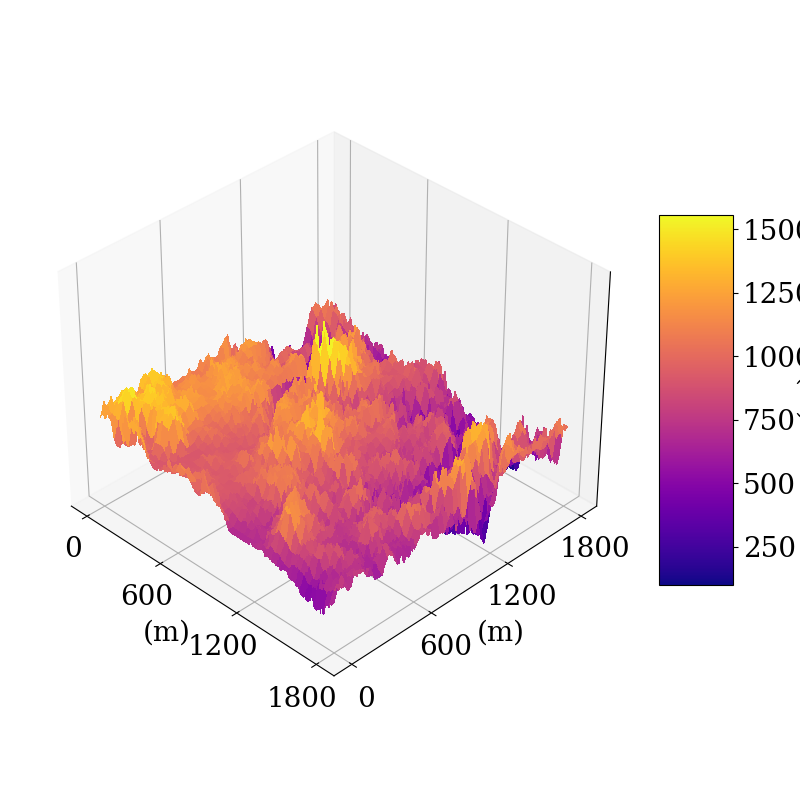
\includegraphics[width=1.0\textwidth]{../runsAndAdditions/realdata3D.png}
%         \caption{True Function}\label{fig:realdata3D}
% \end{center}
% \end{minipage}
% \hspace{2mm}
% \begin{minipage}[!t]{.48\linewidth}
%     \begin{center}
%         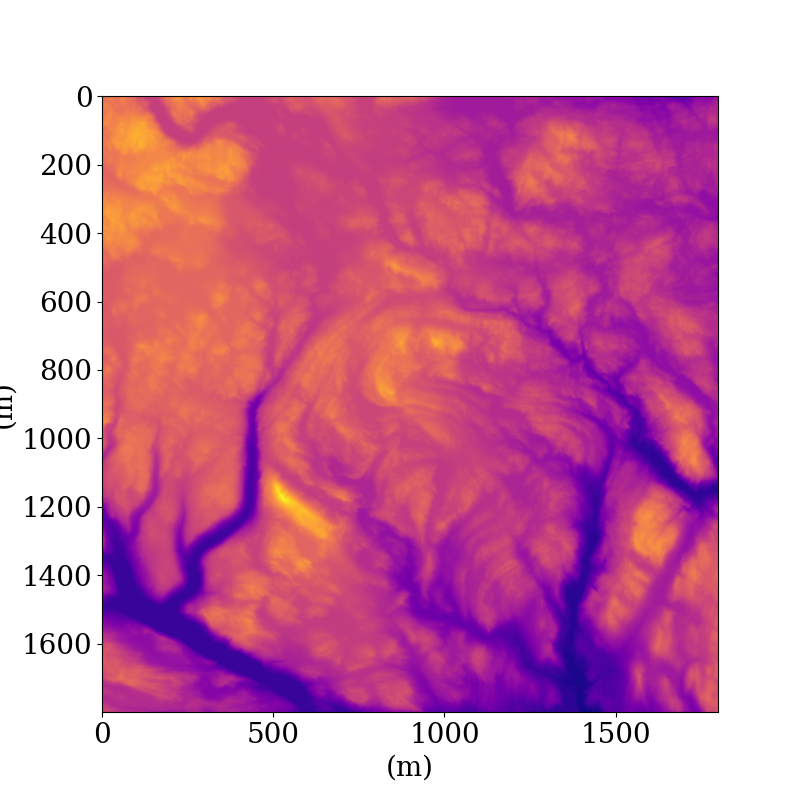
\includegraphics[width=1.0\textwidth]{../runsAndAdditions/realdataMap.png}
%         \caption{Our Synthetic Data}\label{fig:realdataMap}
%     \end{center}
% \end{minipage}
% \end{figure}
% The noise is sampled from a normal distribution with mean 0 and standard deviation $\sigma = 0.1$.
% The data is generated by sampling x and y from a uniform distribution on the interval \[0, 1\].
% This synthetic data is divided into training and testing sets, with the testing set comprising twenty percent and the training set comprising eighty percent of the total data.
% In addition, we will incorporate genuine topographic data from a specific area of Norway. However, to reduce computational requirements when running the program, we've reduced the size of this real topographic dataset from 6.5 million points to 10,000 points.




\section{Results and Discussion}
\label{sec:resultsdiscussion}








% \section{Bias \& Variance}
% \label{sec:biasvariance}



\section{Conclusion}
\label{sec:conclusion}






















% \acks{}



% APPENDIX

%
%
\newpage
\appendix
\phantomsection%
\addcontentsline{toc}{section}{Appendix}
\section*{Appendix}
\label{app:appendix}




\phantomsection%
\addcontentsline{toc}{subsection}{ Lines glued together }
\subsection*{Lines glued together $\boldsymbol{\beta}$}
\label{app:OptimalBeta}




\phantomsection%
\addcontentsline{toc}{subsection}{ learn xor with perceptron }
\subsection*{Lines glued together $\boldsymbol{\beta}$}
\label{app:OptimalBeta}


% \phantomsection%
% \addcontentsline{toc}{subsection}{SVD}
% \subsection*{SVD}
% \label{app:svd}





% \phantomsection%
% \addcontentsline{toc}{subsection}{Confidence Interval}
% \subsection*{Math Behind the Confidence Interval, Section~\ref{sec:confidenceinterval}}
% \label{app:confidenceinterval}




\vskip 0.2in
\bibliography{report}
% \bibliographystyle{apalike}
\bibliographystyle{plain}
\phantomsection%
\addcontentsline{toc}{section}{Bibliography}
\end{document}








